\documentclass{article}
\usepackage[margin=1in]{geometry}
\usepackage{graphicx}
\usepackage{hyperref,fancyvrb,amsmath}
\usepackage{tikz}
\usepackage{tikz-qtree}

\newcommand{\mydot}[1]{\draw[fill] (#1) circle (0.1);}

\newcommand{\set}[1]{\ensuremath{\{#1\}}}

\title{CSCI 241, Project \#3, Random Maze Generation}
\author{Geoffrey Matthews}

\begin{document}

\maketitle

\centerline{\bf Note:  This is still incomplete.}


\centerline{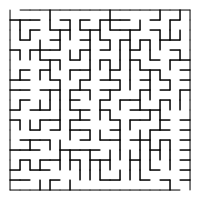
\includegraphics[scale=0.5]{maze.png}}



\begin{description}

\item[Due date:] Midnight, May 26.

\item[Turn in:] Be sure to {\bf zip} all your source files together
  before submission.  Canvas downloads mangle the names, and java
  likes to have the names of the files the same as the public class in
  the file.

  To make
  it easier for me to write scripts to unpack, compile, and run your
  file:
  \begin{itemize}
    \item
      Use {\bf zip}, not tar or 7z or any other archiving software.
      \item Zip the folder, not the individual  files in the folder.
      \item Name the zip file {\tt lab03.zip}.
\item
  Nmae the file (and class) with your {\tt main} method in it {\tt
    lab03.java}. 
  \end{itemize}

\item[Input and output:]  The number of rows and the number of
  columns as arguments.  The output will be a graphical image of the
  maze (see the java example from the previous lab to see how to make
  images). 
  
\item[Maze algorithm:] To draw a maze, consider a rectangular grid
  with each cell labelled and walls between all adjacent cells. as in
  Figure \ref{mazefig} (a).  In the beginning, we regard each cell as
  in its own set by itself (since it is separated from the others by
  walls).  Thus, we have a {\em partition} of the set of $n$ cells
  into $n$ sets.  We will now gradually reduce the size of this
  partition to 1 by merging two sets at a time.

  We pick two adjacent cells from different sets at random, for
  example, 4 and 9.  We put a door (remove the wall) between them,
  merging their sets and getting Figure \ref{mazefig} (b), and we now
  have 24 sets of cells, all the sets not including 4 or 9, and the
  set \set{4,9}.

  We now pick another pair of adjacent cells at random, which are in
  {\em different} sets, for example 3 and 4, and put a door (remove a
  wall) between them.  This merges the sets \set{3} and the set
  \set{4,9} into the set \set{3,4,9}, and results in Figure
  \ref{mazefig} (c).


  Now we pick a different pair of random adjacent cells from different
  sets, for example 20 and 21, put a door between them and merge their
  sets, giving Figure
  \ref{mazefig} (d).


  We continue in this fashion, each time removing a wall between two
  random {\em adjacent} cells that are in {\em different} sets,
  merging the sets,  until
  we have only one set remaining, as in Figure \ref{mazefig} (e).  


At this point, we have a maze if we just remove the cell labels
and leave an entrance at the upper left, and an
exit at the lower right, as in Figure \ref{mazefig} (f).
  
It is crucial that we always pick a pair of adjacent cells from {\em
  different} sets.  If they are not adjacent putting a door between
them makes no sense.  If they are in the same partition, our maze
would have cycles in it.


\item[Picking random adjacent cells:] As the algorithm progresses,
  there will be fewer and fewer adjacent cells in different
  partitions.  If we just pick cells at random, it will take longer
  and longer to find a candidate to merge.  To solve this we take the
  following approach.

  Before we begin, we form a complete list of all adjacent cell pairs.
  Each cell in the range (0\ldots n-2) is paired up with the cells to
  the right and below it, if they exist.  For example, for the cells
  in Figure \ref{mazefig}, the list would start out looking like this:
  \[
  ((0,1), (0,5), (1,2), (1,6), (2,3), (2,7), (3,4), (3,8), (4,9),
  (5,10), \ldots, (21,22), (22,23), (23,24) )
  \]
  Note that some cells (on the right side and the bottom) have only
  one adjacent cell, and the last cell has no adjacent cell.

  Now we randomize this list.  The algorithm is simple:  for each
  pair of cells, swap that pair with a pair at a random location.

  We use this list every time we want a new pair of random cells.  We
  remove the first pair and check to see if the two cells are in
  different partitions.  If they are in different partitions, we put a
  door there and merge the partitions.  We put this pair in another
  list ({\em e.g.}, {\tt doors}).  If we don't put a door there (they were
  in the same partition), we keep them in a different list ({\em
    e.g.}, {\tt walls}).

  We can now use the list of {\tt walls} to tell us where all the
  internal walls are drawn in the final maze.  Having this list makes
  it easy to draw the final maze: draw the outside border (leaving the
  entrance and exit open), and then draw a wall segment between each
  pair of cells in the {\tt walls} list.

\item[Merging  and detecting disjoint sets:]
  
Now that we have a random pair of cells, another problem is maintaining
the partition of the cells, with the following operations as fast as
possible: 
  \begin{itemize}
  \item Determine if two cells are in the same partition.
    \item Merge two partitions into one.
  \end{itemize}

If we do this inefficiently, every time we have two cells, $i$ and
$j$, and want to know if they are in the same set, we may have to use
an $O(n)$ process to find this out.  We can do a lot better than that.

  To accomplish this, wére going to use a forest of trees to represent
  the partition.  We are going to have to insert and delete trees from
  this forest, so pick an efficient data structure for that, but the
  order is not going to matter.

  We are also going to have to quickly find a node in the tree, given
  just its index, so keep an array $(0,\ldots,n-1)$ of pointers to the
  individual nodes in the forest as well.

For these trees we are only going to use {\em parent} pointers, and
they will be general trees, not binary trees.  (The data structure
looks a lot like a linked list, but we're going to use it as if it
were a tree.)

  Each cell starts out in its own tree, as in Figure \ref{mergesets}
  (a).  In order to merge cells 4 and 9, we simply make the root of
  one the parent of the root of the other; for example as in Figure
  \ref{mergesets} (b), where we made 9 the parent of 4.  In (c) we
  join 3 and 4 by merging \set{3} with \set{4,9}, by making 9 the
  parent of 3 (since 9 is the root of \set{4,9}).  The next few merges
  are shown in Figure \ref{mergesets} (d) to (h).  (Which cells were
  merged at each step?)

Clearly, given two cells, merging their sets is a fast operation.  We
merely find their roots, and then make the root of one be the parent
of the other.

But what about determining if two nodes are in the same partition?

The beauty here is that it is going to be very fast to find the root
of each cell's tree.  Two cells are in the same set if they have the
same root.  For example, in Figure \ref{mergesets} (h), cells 3 and 20
are in different sets, because $\mbox{root}(3) = 19 \not =
21 = \mbox{root}(20) $.




\end{description}

\begin{figure}
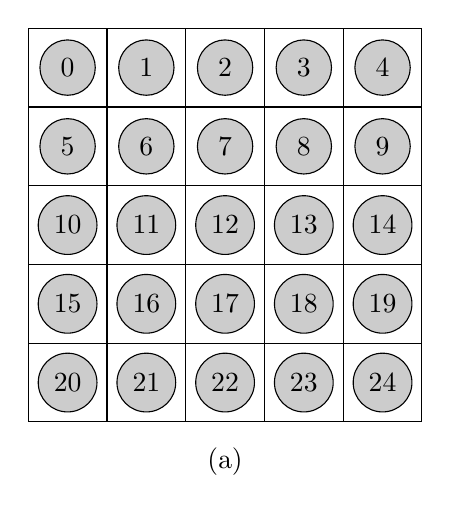
\begin{tikzpicture}[scale=1.0,darkstyle/.style={circle,draw,fill=gray!40,minimum size=20}]
  \foreach \x in {0,...,4}
    \foreach \y in {0,...,4} 
       {\pgfmathtruncatemacro{\label}{\x - 5 *  \y +20}
       \node [darkstyle]  (\x\y) at (0.5+\x,0.5+\y) {\label};} 

 \draw (5,0) -- (5,5) -- (0,5);
  \foreach \x in {0,...,4}
    \foreach \y in {0,...,4}
      \draw (\x, \y) -- (1+\x, \y)
            (\x, \y) -- (\x, 1+\y)
      ;
 \draw  (2.5,-0.5) node {(a)};
\end{tikzpicture}\hfill
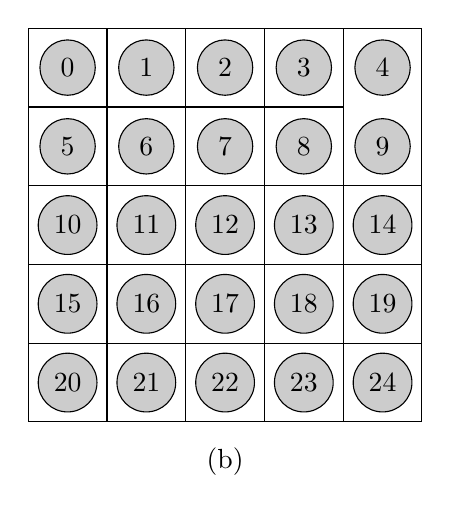
\begin{tikzpicture}[scale=1.0,darkstyle/.style={circle,draw,fill=gray!40,minimum size=20}]
  \foreach \x in {0,...,4}
    \foreach \y in {0,...,4} 
       {\pgfmathtruncatemacro{\label}{\x - 5 *  \y +20}
       \node [darkstyle]  (\x\y) at (0.5+\x,0.5+\y) {\label};} 

 \draw (5,0) -- (5,5) -- (0,5) -- (0,0) -- cycle;
  \foreach \x in {0,...,4}
    \foreach \y in {0,...,3}
      \draw (\x, \y) -- (1+\x, \y)
            (\x, \y) -- (\x, 1+\y)
      ;
    \foreach \x in {0,...,4}
       \draw (\x,4) -- (\x,5);
    \foreach \x in {0,...,3}
       \draw (\x,4) -- (1+\x,4);
 \draw  (2.5,-0.5) node {(b)};
\end{tikzpicture}\hfill
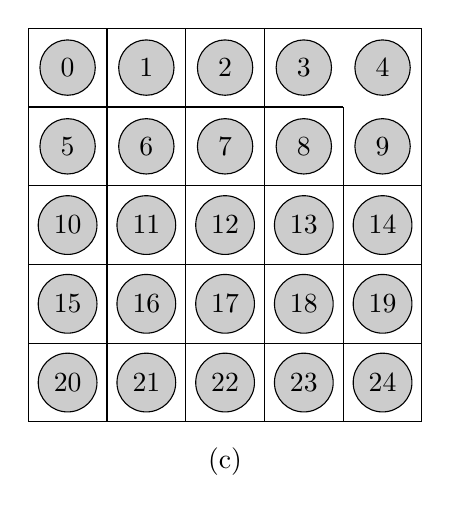
\begin{tikzpicture}[scale=1.0,darkstyle/.style={circle,draw,fill=gray!40,minimum size=20}]
  \foreach \x in {0,...,4}
    \foreach \y in {0,...,4} 
       {\pgfmathtruncatemacro{\label}{\x - 5 *  \y +20}
       \node [darkstyle]  (\x\y) at (0.5+\x,0.5+\y) {\label};} 

 \draw (5,0) -- (5,5) -- (0,5) -- (0,0) -- cycle;
  \foreach \x in {0,...,4}
    \foreach \y in {0,...,3}
      \draw (\x, \y) -- (1+\x, \y)
            (\x, \y) -- (\x, 1+\y)
      ;
    \foreach \x in {0,...,3}
       \draw (\x,4) -- (\x,5);
    \foreach \x in {0,...,3}
       \draw (\x,4) -- (1+\x,4);
 \draw  (2.5,-0.5) node {(c)};
\end{tikzpicture}

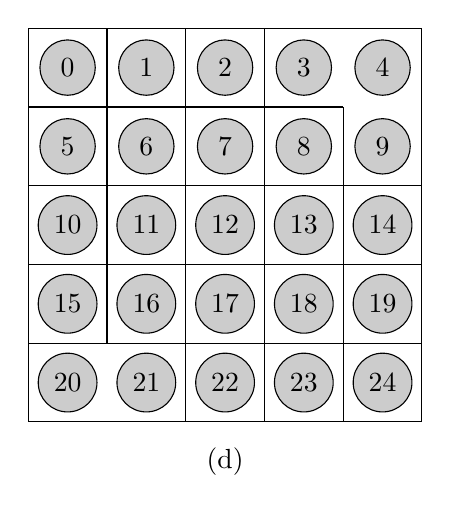
\begin{tikzpicture}[scale=1.0,darkstyle/.style={circle,draw,fill=gray!40,minimum size=20}]
  \foreach \x in {0,...,4}
    \foreach \y in {0,...,4} 
       {\pgfmathtruncatemacro{\label}{\x - 5 *  \y +20}
       \node [darkstyle]  (\x\y) at (0.5+\x,0.5+\y) {\label};} 

 \draw (5,0) -- (5,5) -- (0,5) -- (0,0) -- cycle;
  \foreach \x in {0,...,4}
    \foreach \y in {1,...,3}
      \draw (\x, \y) -- (1+\x, \y)
            (\x, \y) -- (\x, 1+\y)
      ;
    \foreach \x in {0,...,3}
       \draw (\x,4) -- (\x,5);
    \foreach \x in {0,...,3}
    \draw (\x,4) -- (1+\x,4);
    \foreach \x in {2,...,4}
    \draw (\x,0) -- (\x,1);
 \draw  (2.5,-0.5) node {(d)};
\end{tikzpicture}\hfill
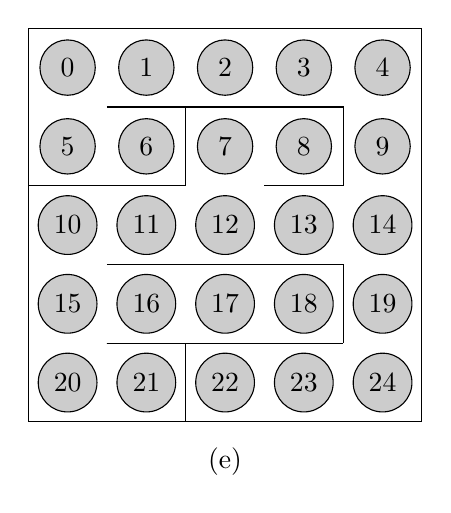
\begin{tikzpicture}[scale=1.0,darkstyle/.style={circle,draw,fill=gray!40,minimum size=20}]
  \foreach \x in {0,...,4}
    \foreach \y in {0,...,4} 
       {\pgfmathtruncatemacro{\label}{\x - 5 *  \y +20}
       \node [darkstyle]  (\x\y) at (0.5+\x,0.5+\y) {\label};} 

 \draw (5,0) -- (5,5) -- (0,5) -- (0,0) -- cycle;
 \draw (2,0) -- (2,1) -- (1,1) -- (2,1) -- (3,1) -- (4,1)
       (1,2) -- (2,2) -- (3,2) -- (4,2) -- (4,1)
       (0,3) -- (1,3) -- (2,3) -- (2,4) -- (1,4)
       (1,4) -- (2,4) -- (3,4) -- (4,4) -- (4,3) -- (3,3)
 ;
 \draw  (2.5,-0.5) node {(e)};
\end{tikzpicture}\hfill
\begin{tikzpicture}[scale=1.0,darkstyle/.style={circle,draw,fill=gray!40,minimum size=20}]

 \draw (1,5) -- (5,5) -- (5,0) (4,0) -- (0,0) -- (0,5);
 \draw (2,0) -- (2,1) -- (1,1) -- (2,1) -- (3,1) -- (4,1)
       (1,2) -- (2,2) -- (3,2) -- (4,2) -- (4,1)
       (0,3) -- (1,3) -- (2,3) -- (2,4) -- (1,4)
       (1,4) -- (2,4) -- (3,4) -- (4,4) -- (4,3) -- (3,3)
 ;
 \draw  (2.5,-0.5) node {(f)};
\end{tikzpicture}
\caption{Merging cells to make a maze.  The original partition is (a),
after merging \set{4} and \set{9} we get (b), after merging \set{3}
and \set{4,9} we get (c), and after merging \set{20} and \set{21} we
get (d).  A full merge down to one set is shown in (e), and drawn as a
maze in (f).}
\label{mazefig}
\end{figure}


  \begin{figure}

(a)  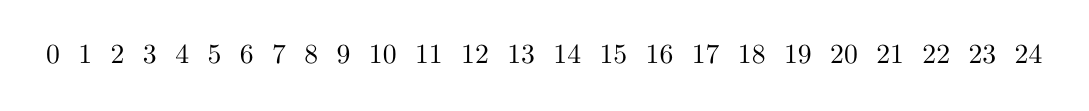
\begin{tikzpicture}
    \matrix {
  \Tree [.0 ] &
  \Tree [.1 ] &
  \Tree [.2 ] &
  \Tree [.3 ] &
  \Tree [.4 ] &
  \Tree [.5 ] &
  \Tree [.6 ] &
  \Tree [.7 ] &
  \Tree [.8 ] &
  \Tree [.9 ] &
  \Tree [.10 ] &
  \Tree [.11 ] &
  \Tree [.12 ] &
  \Tree [.13 ] &
  \Tree [.14 ] &
  \Tree [.15 ] &
  \Tree [.16 ] &
  \Tree [.17 ] &
  \Tree [.18 ] &
  \Tree [.19 ] &
  \Tree [.20 ] &
  \Tree [.21 ] &
  \Tree [.22 ] &
  \Tree [.23 ] &
  \Tree [.24 ] \\
};
\end{tikzpicture}

      \hrulefill
      
(b)  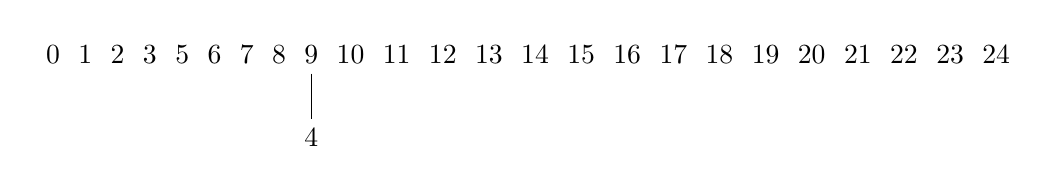
\begin{tikzpicture}
    \matrix {
  \Tree [.0 ] &
  \Tree [.1 ] &
  \Tree [.2 ] &
  \Tree [.3 ] &
  \Tree [.5 ] &
  \Tree [.6 ] &
  \Tree [.7 ] &
  \Tree [.8 ] &
\Tree [.9  [.4 ] ] &
  \Tree [.10 ] &
  \Tree [.11 ] &
  \Tree [.12 ] &
  \Tree [.13 ] &
  \Tree [.14 ] &
  \Tree [.15 ] &
  \Tree [.16 ] &
  \Tree [.17 ] &
  \Tree [.18 ] &
  \Tree [.19 ] &
  \Tree [.20 ] &
  \Tree [.21 ] &
  \Tree [.22 ] &
  \Tree [.23 ] &
  \Tree [.24 ] \\
};
\end{tikzpicture}

      \hrulefill
      

(c)  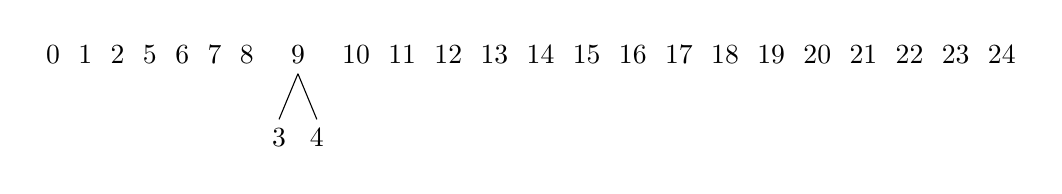
\begin{tikzpicture}
    \matrix {
  \Tree [.0 ] &
  \Tree [.1 ] &
  \Tree [.2 ] &
  \Tree [.5 ] &
  \Tree [.6 ] &
  \Tree [.7 ] &
  \Tree [.8 ] &
\Tree [.9  [.3 ] [.4 ] ] &
  \Tree [.10 ] &
  \Tree [.11 ] &
  \Tree [.12 ] &
  \Tree [.13 ] &
  \Tree [.14 ] &
  \Tree [.15 ] &
  \Tree [.16 ] &
  \Tree [.17 ] &
  \Tree [.18 ] &
  \Tree [.19 ] &
  \Tree [.20 ] &
  \Tree [.21 ] &
  \Tree [.22 ] &
  \Tree [.23 ] &
  \Tree [.24 ] \\
};
\end{tikzpicture}


      \hrulefill
      


(d)  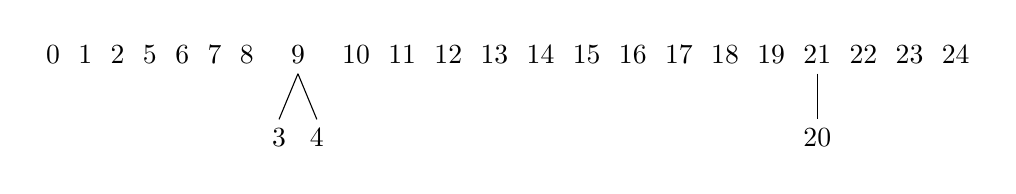
\begin{tikzpicture}
    \matrix {
  \Tree [.0 ] &
  \Tree [.1 ] &
  \Tree [.2 ] &
  \Tree [.5 ] &
  \Tree [.6 ] &
  \Tree [.7 ] &
  \Tree [.8 ] &
\Tree [.9  [.3 ] [.4 ] ] &
  \Tree [.10 ] &
  \Tree [.11 ] &
  \Tree [.12 ] &
  \Tree [.13 ] &
  \Tree [.14 ] &
  \Tree [.15 ] &
  \Tree [.16 ] &
  \Tree [.17 ] &
  \Tree [.18 ] &
  \Tree [.19 ] &
  \Tree [.21 [.20 ] ] &
  \Tree [.22 ] &
  \Tree [.23 ] &
  \Tree [.24 ] \\
    };
  \end{tikzpicture}

      \hrulefill
      


(e)  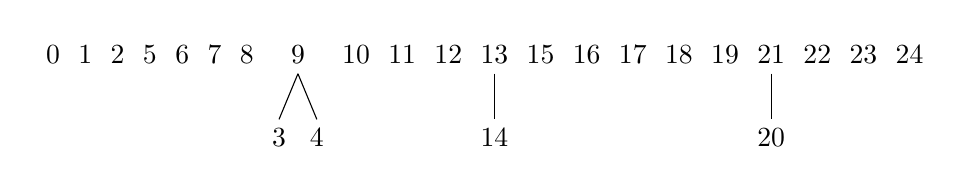
\begin{tikzpicture}
    \matrix {
  \Tree [.0 ] &
  \Tree [.1 ] &
  \Tree [.2 ] &
  \Tree [.5 ] &
  \Tree [.6 ] &
  \Tree [.7 ] &
  \Tree [.8 ] &
\Tree [.9  [.3 ] [.4 ] ] &
  \Tree [.10 ] &
  \Tree [.11 ] &
  \Tree [.12 ] &
  \Tree [.13 [.14 ] ] &
  \Tree [.15 ] &
  \Tree [.16 ] &
  \Tree [.17 ] &
  \Tree [.18 ] &
  \Tree [.19 ] &
  \Tree [.21 [.20 ] ] &
  \Tree [.22 ] &
  \Tree [.23 ] &
  \Tree [.24 ] \\
    };
  \end{tikzpicture}


      \hrulefill
      

(f)  \begin{tikzpicture}
    \matrix {
  \Tree [.0 ] &
  \Tree [.1 ] &
  \Tree [.2 ] &
  \Tree [.5 ] &
  \Tree [.6 ] &
  \Tree [.7 ] &
  \Tree [.8 ] &
\Tree [.9  [.3 ] [.4 ] [.13 [.14 ] ] ] &
  \Tree [.10 ] &
  \Tree [.11 ] &
  \Tree [.12 ] &
  \Tree [.15 ] &
  \Tree [.16 ] &
  \Tree [.17 ] &
  \Tree [.18 ] &
  \Tree [.19 ] &
  \Tree [.21 [.20 ] ] &
  \Tree [.22 ] &
  \Tree [.23 ] &
  \Tree [.24 ] \\
    };
  \end{tikzpicture}


      \hrulefill
      


(g)  \begin{tikzpicture}
    \matrix {
  \Tree [.0 ] &
  \Tree [.1 ] &
  \Tree [.2 ] &
  \Tree [.5 ] &
  \Tree [.6 ] &
  \Tree [.7 ] &
  \Tree [.8 ] &
  \Tree [.10 ] &
  \Tree [.11 ] &
  \Tree [.12 ] &
  \Tree [.15 ] &
  \Tree [.16 ] &
  \Tree [.17 ] &
  \Tree [.18 ] &
  \Tree [.19 [.9  [.3 ] [.4 ] [.13 [.14 ] ] ]   ] &
  \Tree [.21 [.20 ] ] &
  \Tree [.22 ] &
  \Tree [.23 ] &
  \Tree [.24 ] \\
    };
  \end{tikzpicture}



      \hrulefill
      

(h)  \begin{tikzpicture}
    \matrix {
  \Tree [.0 ] &
  \Tree [.1 ] &
  \Tree [.2 ] &
  \Tree [.5 ] &
  \Tree [.6 ] &
  \Tree [.7 ] &
  \Tree [.8 ] &
  \Tree [.10 ] &
  \Tree [.11 ] &
  \Tree [.12 ] &
  \Tree [.15 ] &
  \Tree [.16 ] &
  \Tree [.17 ] &
  \Tree [.18 ] &
  \Tree [.19 [.9  [.3 ] [.4 ] [.13 [.14 ] ] ] [.24 ]  ] &
  \Tree [.21 [.20 ] ] &
  \Tree [.22 ] &
  \Tree [.23 ] \\
    };
  \end{tikzpicture}



  \caption{Merging sets with trees.  Which two cells are merged at
    each stage? }
  \label{mergesets}
  \end{figure}

\end{document}
